\section{Known Bugs}
\label{teila_knownbugs}
Im Laufe der Arbeit gab es Erschwernisse, welche die Entwicklung verzögerten. 
Als Einschränkung bezüglich des \code{MD050SD}, stellt sich die begrenzte Geschwindigkeit von 50~MHz dar. Mit einer maximalen Busgeschwindigkeit von 90~MHz des LPC3131 könnte das Display wesentlich schneller betrieben werden, was die Framerate fast verdoppeln würde. Zusätzlich erscheinen auf dem Display zufällig Artefakte in Form von einzelnen Pixeln. Dies lässt die Vermutung zu, dass die Leitungen von der Adapterplatine oder des \code{MD050SD} selbst anfällig für Störungen von außen sein können. \\ \\
Bezüglich dem \code{SSD1289} stellte sich heraus, dass die Verwendung der angebotenen Kommandos aus \reft{tab:Kommandos_SSD1289} nicht für die Adressierung eines RAM-Fensters über mehrere Zeilen zuverlässig funktioniert. Unabhängig vom gesendeten Kommando treten zufällig Resets des Displaycontrollers auf, welche das Display nach kurzer Zeit komplett weiß erscheinen lässt. Als Lösung besteht die Möglichkeit der Reservierungen einzelner Zeilen, die in der Summe das komplette RAM-Fenster abdecken. Nachteilig stellt sich hierbei der erhöhte Adressierungsaufwand dar, da jede Zeile erneut adressiert werden muss.\\ \\
Der Betrieb mit dem \code{SSD1963} ist problematischer als anfangs angenommen. Die Ursache des Problems ist noch ungeklärt, was den Betrieb mit dem \code{SSD1963} derzeit unmöglich macht.
Das Problem stellt sich so dar, dass sich trotz scheinbar korrektem Datenverkehr auf dem 8080-Bus der Displaycontroller nicht initialisieren lässt. Als erster Schritt der Initialisierung steht die PLL\footnote{PLL: Phase Locked Loop, Phasenregelschleife zur Erzeugung von hohen Taktraten}. Mithilfe der PLL wird der erforderliche Displaytakt von z.~B. 90~MHz erzeugt und der Controller mit dieser Frequenz betrieben. Solch ein schneller Zugriff auf den \code{SSD1963} ist erst nach der Initialisierung der PLL möglich. Bevor dies der Fall ist, kann mit maximal 5 M Words/s \footnote{5M~Word/s: $5*10^6$ Datenwörter pro Sekunde} geschrieben bzw. gelesen werden (siehe \cite{SSD2008}, S. 72). Um den Fehler zu finden, wurden diverse Überlegungen angestellt. Angedachte potentielle Fehlerquellen sind
\begin{itemize}
\item zu flache Flanken der Signale
\item 8080-Bus Protokoll nicht eingehalten
\item 8080-Bus Timing nicht im Rahmen der Spezifikationen des \code{SSD1963}
\item 8080-Bus Datenverkehr fehlerhaft
\item Leitungsführung auf dem Display selbst schlecht
\end{itemize}
Die Flanken der Signale haben sich nach Messungen mit dem Oszilloskop als nicht zu flach herausgestellt und können als Fehlerquelle ausgeschlossen werden. Die Einhaltung des 8080-Bus Protokolls sowie der Timings wurden ebenfalls überprüft. Hierzu ist dasselbe Display mit einer funktionierenden Displayansteuerung über die \code{GPIO}-Pins aufgebaut und jedes Kommando der Initialisierung des \code{SSD1963} mit dem Logic-Analyzer aufgenommen worden. Derselbe Displaytreiber, mit dem Unterschied der Ansteuerung über das SRAM-Interface, wurde ebenfalls aufgezeichnet und mit den Daten der vorhergehenden Messung verglichen. Diese Methode schließt einen fehlerhaften Datenverkehr aus und lässt zusätzlich die Rahmenbedingungen für das 8080-Interface selbst und dessen Timing überprüfen. Für die Aufzeichnung, wurde der User-Space-Treiber dahingehend modifiziert, dass er vor dem Senden die Bestätigung des Anwenders abfragt. Die Abbildungen \ref{fig:ssd1963_gpio} und \ref{fig:ssd1963_sram} zeigen einen exemplarischen Datentransfer für die beiden Ansteuerungsmethoden. Zu erkennen ist, dass dasselbe Wort an den Datenpins \code{D[7:0]} anliegt, und die Steuersignale \code{CS}, \code{WR}, \code{RD} und \code{A15} innerhalb der markierten Zonen entsprechend dem 8080-Interface geschaltet werden. 

\begin{figure}[htp]
        \begin{center}
        \begin{subfigure}[htp]{1\textwidth}
			%\begin{figure}[h!]
			\centering
			\fbox{	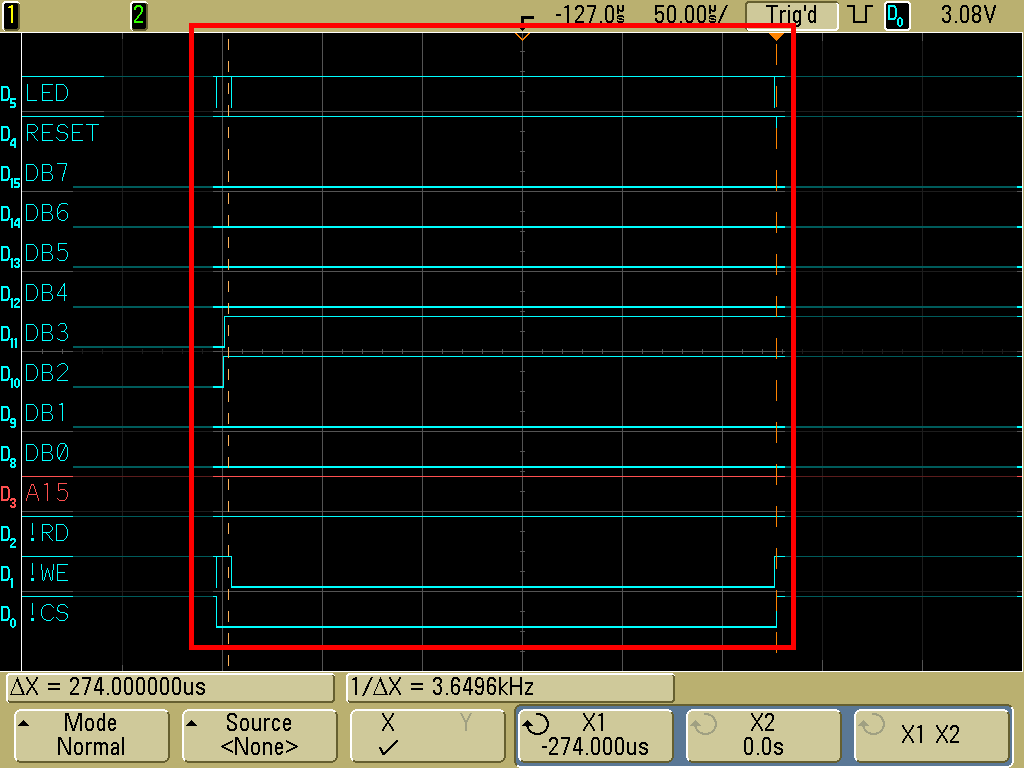
\includegraphics[width=1\textwidth]{TeilA/print_34_dip.png}}
	\caption{SSD1963 mit GPIO}
			\label{fig:ssd1963_gpio}
		\end{subfigure}


        \begin{subfigure}[htp]{1\textwidth}
%\begin{figure}[h!]
	\centering
\fbox{	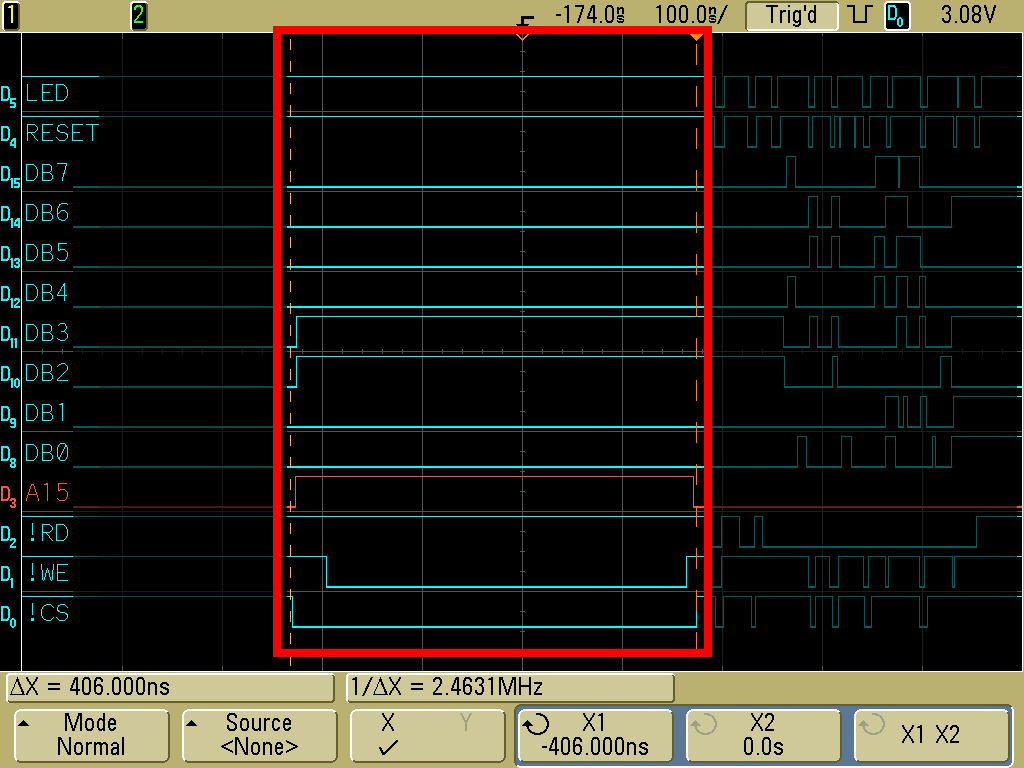
\includegraphics[width=1\textwidth]{TeilA/print_34_ext.png}}
	\caption{SSD1963 mit SRAM-Interface}
	\label{fig:ssd1963_sram}
\end{subfigure}

		\end{center}
\caption{SSD1963: Vergleich GPIO- und SRAM-Ansteuerung}
	\label{fig:ssd1963_gpio_sram}
\end{figure}

\newpage
Das geforderte Timing des Displays ist in \refa{fig:ssd1963_timing_constraints} zu sehen und beinhaltet die minimal notwendigen Zeiten zwischen den einzelnen Signalen.
\begin{figure}[htp]
%\begin{minipage}[t]{0.8\textwidth}
%\begin{figure}[h]
	\centering
\fbox{	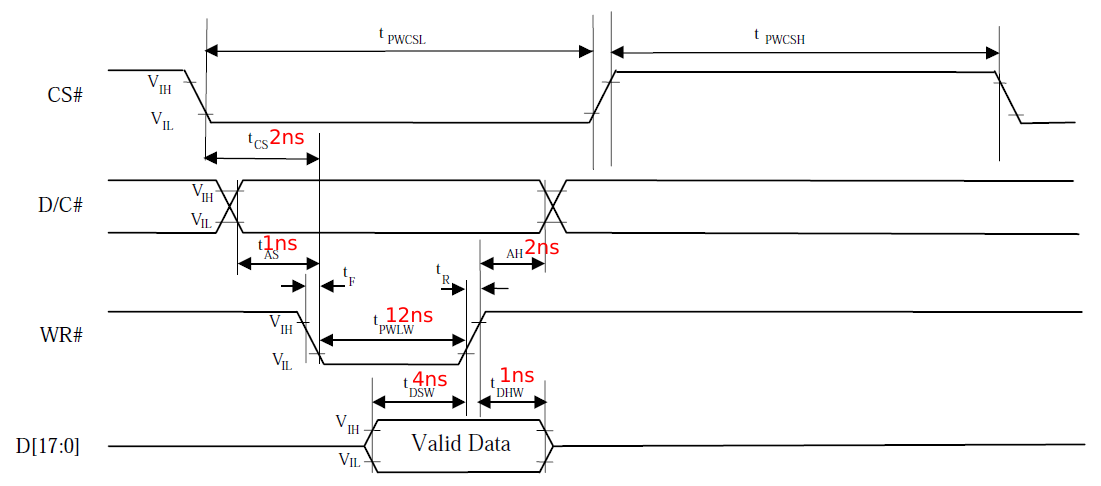
\includegraphics[width=1.0\textwidth]{TeilA/ssd1963_writeCycleConstraings.png}}
	\caption{8080-Timingbedingung für SSD1963}
	\label{fig:ssd1963_timing_constraints}
\end{figure}\newline
Diese Mindestzeiten wurden innerhalb der Oszilloskopbilder eingehalten und verifiziert, sodass ein Fehler mit dem Protokoll des 8080-Interface ausgeschlossen werden kann. Bezüglich der uninitialisierten PLL des Displays und der verringerten Schreibrate ist in \refa{fig:ssd1963_sram} eine Chip-Select-Länge von 406~Nanosekunden erkennbar. Dies entspricht einer Schreibgeschwindigkeit von 2.46~MHz. Die Frequenz ist weit unter den geforderten 5~MHz im uninitialisierten Zustand. Deshalb ist ein zu schnelles Schreiben in diesem Fall ebenfalls ausgeschlossen. Nachdem verifiziert wurde, dass aus der Adapterplatine vom \code{Gnublin Extended} die richtigen Signale geliefert werden, bleibt als vermutete Ursache nur noch das Display selbst. Da die Leitungsführung des ursprünglich verwendeten 4.3 Zoll Displays nicht optimal ist, wurde der Fehler im schlechten Platinendesign des Displays gesucht.
Dort sind die 8080-Leitungen quer über die Platine geführt und im Anschluss von den RGB-Signalen im 90 Grad Winkel gekreuzt. Aufgrund dessen fand das 5 Zoll Display mit demselben Controller Verwendung, welches eine optimierte Leitungsführung besitzt. Jedoch waren die aufgeführten Lösungsansätze nicht zielführend, weswegen das Display nicht mit dem \code{Gnublin Extended} unter Verwendung des SRAM-Interface einsetzbar ist.